%---------------------------------------------------
% Integration
%---------------------------------------------------
\chapter[Integration]{Integration $<\int>$}
In mathematics we are often given a function $f$ and asked to find a function $F$ whose derivative is $f$. $\;F$ in this situation is called the integral of $f$. It is usual to develop a list of integrals by differentiating a range of functions then using those to work backwards. The terms integration and anti-differentiation are synonymous. Generally we will use the term integration, however, both are acceptable.

The process of `reversing' or `undoing' a derivative has its own symbol, the integrand: $\displaystyle\int$
\begin{tcolorbox}
	\[\int f'(x) dx = f(x)+C\]
\end{tcolorbox}

%---------------------------------------------------
% Standard Integrals
%---------------------------------------------------
\section{Standard Integrals}
It is not the intention here to list all of the rules that are required however at this stage let us explore the Power Rule to establish a rule for integrating an expression of the form $y =x^{n}$ \\

\begin{center}
\begin{tabular}[c]{p{1.5cm}p{1.5cm}}\toprule
function $f(x)$  & derivative $f'(x)$  \\
\midrule
$x$  & $1$  \\
$x^{2}$  & $2 x$  \\
$x^{3}$  & $3 x^{2}$  \\
$x^{4}$  & $4 x^{3}$  \\
\bottomrule
\end{tabular}\ or
\
\begin{tabular}[c]{ll}\toprule
 $f$  & $f'$  \\
 &\\
\midrule
$x$  & $1$  \\
$\frac{1}{2} x^{2}$  & $x$  \\
$\frac{1}{3} x^{3}$  & $x^{2}$  \\
$\frac{1}{4} x^{4}$  & $x^{3}$  \\
\bottomrule
\end{tabular}\ now, in reverse \
\begin{tabular}[c]{p{2cm}p{2.5cm}}\toprule
derivative $f'(x)$  &  integral $\int f'(x)=f(x)$  \\\midrule
$1$  & $x +C$  \\
$x$  & $\frac{1}{2} x^{2} +C$  \\
$x^{2}$  & $\frac{1}{3} x^{3} +C$  \\
$x^{3}$  & $\frac{1}{4} x^{4} +C$  \\
\bottomrule
\end{tabular}
\end{center}
\bigskip This establishes the pattern and if you think about the rule for differentiating $y =x^{n}$ you can soon establish the rule for integrating $x^{n}$.
\begin{tcolorbox}
	The \textbf{Power Rule} for integrating polynomials
\[\int x^n dx = \frac{x^{n +1}}{n +1} +c, \text{ where }n \neq  -1
\]
\end{tcolorbox}

\begin{equation*}\text{ If }f (x) =x^{ -1}\text{ then the integral of }f\text{ is }\ln  \left \vert x\right \vert  +c\text{ or }\ln  \left \vert k x\right \vert
\end{equation*}
All of the differentiation rules we have met so far lead to integration rules. For instance we can establish standards for $\sin  x$, $\cos  x$, and $\sec ^{2} x\text{.}$ The standard integrals are summarized in the table below.
\renewcommand\arraystretch{1.2}
\begin{center}
	\begin{tabular}{llcl}
		\toprule
		Function&Integral&&Notes\\
		$f(x)$  &  $\int f(x)dx$ \\ \midrule
		$1$&$x+C$&&constant\\
		$A$&$Ax+C$&&$A$ is constant\\ \midrule
		$x^n, n \neq -1$ & $\displaystyle\frac{x^{n+1}}{n+1}+C$&&power rule general form\\ 
		$e^x$ & $e^x+C$&&exponential\\ 
		$\frac{1}{x}$ & $\ln|x|+C$&&special case: $x^{-1}$\\
		$\ln x$&$x\ln |x|-x+C$&&\\\midrule
		$\sin(x)$ & $-\cos(x)+C$&& trigonometric \\ 
		$\cos(x)$ & $\sin(x)+C$\\ 
		$\tan (x)$&$\ln |\sec x|+C$\\
		$\sec^2(x)$ & $\tan(x)+C$ \\ \bottomrule
	\end{tabular}
\end{center}

To allow us to combine these integrals and thus extend the range of questions we can tackle we use two important rules for integrals 
\begin{tcolorbox}
\textbf{Sum Rule} The integral of the sum of two functions is the sum of the integrals of the functions.
\[\int \left [f (x) +g (x)\right ]\; d x =\int f (x)\; d x +\int g (x)\; d x\]
\end{tcolorbox}
This is easily extended to the sum or difference of a number of functions. 
\begin{tcolorbox}
\textbf{Constant Multiple Rule} The integral of a constant times a function is the constant times the integral of the function.
\[\int c f (x)\; d x =c \int f (x)\; d x
\]\end{tcolorbox}

\subsection*{Indefinite Integrals}
Although $\int f (x) d x$ looks very similar to $\int _{a}^{b}f (x)\; d x$ they are quite different and must not be confused or used in place of each other. $\int f (x)\; d x$ is a function of $x$ or a family of functions of $x$ and $\int _{a}^{b}f (x)\; d x$ is a number. They are connected of course, provided $f (x)$ is a continuous function of $x$ on $\left [a ,b\right ]$. In this case the Evaluation Theorem gives the connection between them.
\begin{equation*}\int _{a}^{b}f (x)\; d x =\left .\int f (x)\; d x\right ]_{a}^{b}
\end{equation*}

The indefinite integral represents either a particular integral or a family of integrals. These will use a constant $C$ where $C$ takes a different value for each member of the family. $C$ is called the \emph{constant of integration}. 

\example Integrate the following functions; find $\displaystyle\int f(x)$.
\begin{tasks}(2)
	\task $f(x) =3x^{2}$ \medskip\\
	\solution Applying the power rule:\\
\begin{align*}\int 3x^{2}\,dx&=\frac{3x^{2+1}}{2+1}+C\\
	&=x^3+C\end{align*}
\task $f (x) =7$ \medskip \\
\solution Here we are integrating a constant:\\
\[\int 7\,dx=7x+C\]
\task $f(x) =x^{\frac{2}{3}}$ \medskip\\
\solution The power rule still applies to fractional indices:\\
\begin{align*}\int x^{\frac{2}{3}}\,dx&=\frac{x^{\frac{2}{3}+1}}{\frac{2}{3}+1}+C\\
&=\frac{3 x^{5/3}}{5}+C \end{align*}
\task $f (x) =\frac{1}{2 \sqrt{x}} +\frac{1}{\sqrt{2}}$ \medskip\\
\solution Here we need to combine the sum rule and the power rule:\\
\begin{align*}
\int f(x)\,dx &= \int(\frac{1}{2 \sqrt{x}}) \,dx+\int(\frac{1}{\sqrt{2}}) \,dx\\
&=\frac{1}{2}\int x^{-\frac{1}{2}}+\frac{1}{\sqrt{2}}x+C\\
&=\sqrt{x}+\frac{x}{\sqrt{2}}+C
\end{align*}
\end{tasks}
These four examples are all \textit{indefinite} integrals and have an unknown constant in the answer. The following section will introduce definite integrals.\vspace{1cm}\\
\rule{6.8cm}{0.5pt}\\
\example Find $f (x)$ given $f^{ \prime  \prime } (x) =6$\medskip\\
\solution Here we have a \textit{second} derivative, indicated by the double-prime symbol, $f''$. Knowing that $\int f'(x)=f(x)$ we can safely assume that 
\begin{tcolorbox}
	\[\int f''(x) \,dx = f'(x).\]
\end{tcolorbox}
So $f'(x)=\int f''(x) = \int 6 \,dx = 6x+C$. Now we need to integrate a second time to get $f$.
\[\int (6x+C)\,dx=6x^2+Cx+D\]
We end up with two unknown values, $C$ and $D$ as opposed to just a single value.

The previous two examples of equations involving derivatives. Any equation involving derivatives of a function is called a \emph{differential equation}. We will look into this subject in the next chapter. 

\clearpage
%---------------------------------------------------
% Area
%---------------------------------------------------
\section{Area}\begin{multicols}{2}
In this section we attempt to find the area under a curve. That is the area that lies between a curve and the $x$-axis from $x =a$ to $x =b$. The area is bounded by the $x$-axis, a continuous curve $y =f (x)$ and the two vertical lines $x =a$ and $x =b$. This is shown in the figure with the area shaded in. Note the area stops at the axis. Area as calculated by integration is always in reference to the axis.\\
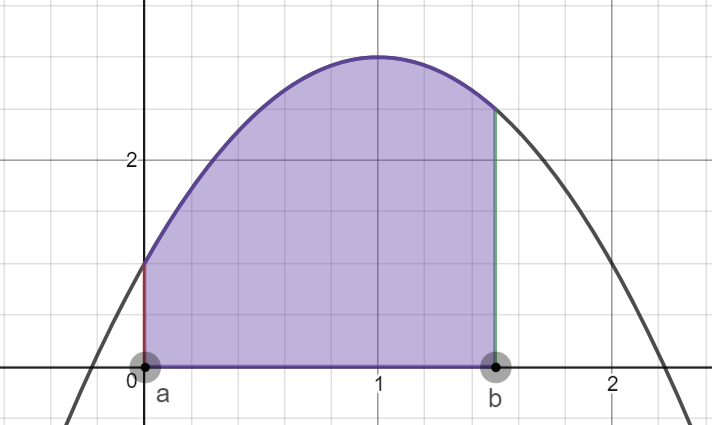
\includegraphics[width=8cm]{area1}
\end{multicols}

Previously, when we wanted to find the slope of a tangent line we found the slope of a secant line and applied the limiting process: $\Lim{h\to 0}$. A similar procedure will be used to find the area. We first approximate the area with rectangular strips then we take the limit of the areas of these rectangular strips by making the strips narrower and narrower and thus the number of strips between $x =a$ and $x =b$ greater and greater. 

\subsection*{Area with Riemann Sums}
\example Given the parabola $y =x^{2}$, use rectangles to find the area under this curve between $0$ and $1$. 

\solution 
\begin{multicols}{2}
\includegraphics[width=8cm]{Area4}\label{fig:riemann}
Consider $4$ strips by constructing vertical lines at $x =\frac{1}{4}, \frac{1}{2}, \frac{3}{4}, \text{and }1$ as shown in the diagram. Rectangles are constructed using the right-hand boundary and we know from inspection this will be larger than the actual area.
\end{multicols}
\begin{align*}
\text{Right sum} &  = \frac{1}{4} \genfrac{(}{)}{}{}{1}{4}^{2} +\frac{1}{4} \genfrac{(}{)}{}{}{1}{2}^{2} +\frac{1}{4} \genfrac{(}{)}{}{}{3}{4}^{2} +\frac{1}{4} \left (1\right )^{2} \\
 &  = \frac{1}{64} +\frac{1}{16} +\frac{9}{64} +\frac{1}{4} \frac{15}{32} =0.46875\end{align*}

Repeating this process with a larger number of rectangles will improve the accuracy of the method. Using a spreadsheet like Excel shows a convergence on a value of $\frac{1}{3}$ as $n$ rectangles increase. The sum using the left-hand boundary is included for comparison.
\begin{center}
	\begin{tabular}[c]{ccc}\toprule
		$n$  & Left sum  & Right sum  \\\midrule
		10		& 0.2850000  & 0.3850000  \\\midrule
		20		& 0.3087500  & 0.3587500  \\\midrule
		30		& 0.3168519  & 0.3501852  \\\midrule
		100		& 0.3283500  & 0.3383500  \\\midrule
		1000	& 0.3328335  & 0.3338335  \\\midrule
		$\infty$& $\frac{1}{3}$&$\frac{1}{3}$\\\bottomrule
\end{tabular}\end{center}
It can be seen that a very accurate approximation to the area can be obtained as the number of rectangles increases. It should be clear that as $n \rightarrow \infty $ both the left sum and the right sum approach the area under the curve we write
\begin{equation*}A =\Lim{n \to \infty}\text{ Left Sum } =\Lim{n \to \infty}\text{ Right Sum }
\end{equation*}
This process can be generalised by selecting any height within each rectangular strip
and finding the area of each strip using this height. Let there be $n$ strips and consider the $i^{t h}$ strip. Select a value of $x$ in the $i^{t h}$ strip call it $x_{i}$. The height of this rectangle will be $f (x_{i})$. Consider the situation described above where the area is bounded by the $x$-axis, a continuous curve $y =f (x)$ and the two vertical lines $x =a$ and $x =b$. 

With $n$ rectangles the length of the base of each rectangle is $ \Delta x =\frac{b -a}{n}$. The area of the $i^{t h}$ rectangle is $f (x_{i})  \Delta x$.

The sum of all the rectangles is
\begin{equation*}\underset{i =1}{\sum ^{n}} f (x_{i})  \Delta x =f \left (x_{1}\right )  \Delta x +f \left (x_{2}\right )  \Delta x +\ldots  +f \left (x_{n}\right )  \Delta x
\end{equation*}

And
\begin{equation*}A =\underset{n \rightarrow \infty }{\lim }\left [\underset{i =1}{\sum ^{n}} f (x_{i})  \Delta x\right ]
\end{equation*}

If $f$ is a continuous function defined on the interval $\left [a ,b\right ]$ then as $n \rightarrow \infty $ the number represented by$\;\underset{i =1}{\sum ^{n}} f (x_{i})  \Delta x \rightarrow A$ the area under the curve $y =f (x)$. This number is called the definite integral of $f$ from $a$ to $b$ and is denoted by $\int _{a}^{b}f$ or $\int _{a}^{b}f (x) d x$
\begin{equation*}\int _{a}^{b}f (x) d x =\underset{n \rightarrow \infty }{\lim }\left [\underset{i =1}{\sum ^{n}} f (x_{i})  \Delta x\right ]
\end{equation*}

This process is called a \emph{Riemann sum} after the German mathematician Bernard Riemann (1826-1866) who defined the integral in this way. The symbol $\int $ was introduced by Leibniz and is called the \emph{integral sign}. 

\subsection*{Definite Integrals}
The method of computing Riemann sums is often long and to achieve a result that is accurate enough requires a computer. Both Isaac Newton and Gottfried Leibniz discovered a much simpler way based on the integral. This discovery is called \emph{The Evaluation Theorem}. 

\begin{tcolorbox}
\textbf{Evaluating Definite Integrals}\\Given $F$ is an integral of $f$ i.e. $F^{ \prime } =f$, provided $f$ is continuous on the interval $[a ,b]$ then 
\[\int _{a}^{b}f (x) d x =F (b) -F (a)\]
\end{tcolorbox}

This is an amazing result in view of the fact that it replaces such a complex procedure as finding
Riemann sums over greater and greater numbers of elementary rectangles. 

\example Evaluate $\int _{0}^{1}x^{2} d x$. 

\solution Because we know a particular integral of $f (x) =x^{2}$ is $F (x) =\frac{1}{3} x^{3}$ We have from the Evaluation Theorem
\begin{equation*}\int _{0}^{1}x^{2} d x =F (1) -F (0) =\frac{1}{3} \cdot 1^{3} -\frac{1}{3} \cdot 0^{3} =\frac{1}{3}
\end{equation*}
Looking back at the calculation of left sum and right sum above we can now see that the actual area
that we were endeavouring to calculate was in fact $1/3$ or $0. \dot{3}$. 

These are some of the different notations for using the Evaluation Theorem 

\begin{equation*}F (b) -F (a) =F (x)\vert _{a}^{b} =\left [F (x)\right ]_{a}^{b} =\left .F (x)\right ]_{a}^{b}
\end{equation*}

\subsection*{Area with Definite Integrals}
Areas above the $x$-axis have \emph{positive} definite integrals and areas below the $x$-axis have \emph{negative} definite integrals. If the context of the question is to evaluate a definite integral then use the definition. If the question is about \textbf{area} you must find the parts of the question that have areas above the $x$-axis and those parts that have areas below the $x$-axis and evaluate them separately. The definite integral calculates the result as the net sum of the positive and negative areas. To find the total area take the absolute value of the individual parts.

\example Find the area under the curve $y =x^{3} -x$ between $x = -1$ and $x =1$.\medskip\\
\begin{SCfigure}[1][h]
	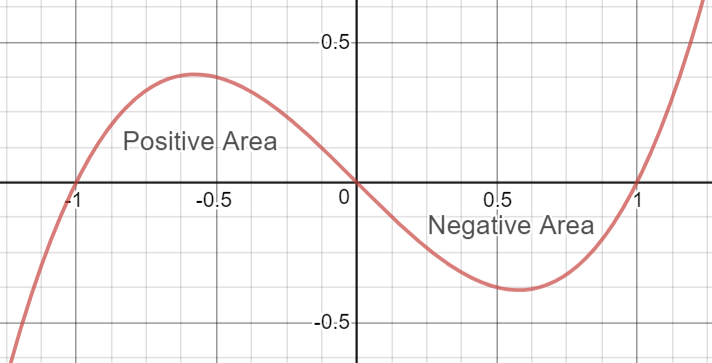
\includegraphics[width=0.6\textwidth]{area3}
	\caption*{Figure: A cubic showing how area `under' the curve is evaluated. The area for $-1\leq x\leq 0$ is positive (above the axis), and the area for $0\leq x\leq 1$ is negative.}
\end{SCfigure}

\solution This can be factored to give $y =x (x +1) (x -1)$. This cubic curve crosses the x-axis at $ -1$, $0$, and $1$. Here, this area must be found in two parts.

\begin{tasks}[column-sep=3ex,label-offset=-5em](3)
	\task[]This is expected to be negative because it is below the axis:\\ 
	$\displaystyle\int _{0}^{1}(x^{3} -x) dx$\\
	$\displaystyle=\frac{x^4}{4}-\frac{x^2}{2}\Big\vert_{0}^1$\\
	$\displaystyle=[\frac{1}{4}-\frac{1}{2}]-0$\\
	$\displaystyle=-\frac{1}{4}$
	\task[]This is expected to be positive:\\ 
	$\displaystyle\int _{ -1}^{0}(x^{3} -x) d x$ \\
	$\displaystyle=\frac{x^4}{4}-\frac{x^2}{2}\Big\vert_{-1}^0$\\
	$\displaystyle=0-[\frac{1}{4}-\frac{1}{2}]$\\
	$\displaystyle=+\frac{1}{4}$
	\task[]Therefore the total area is:\medskip\\
	 $\displaystyle\Big\vert-\frac{1}{4}\Big\vert+\frac{1}{4}=\frac{1}{2}\text{ units}^2$
\end{tasks}
We will compare with a single integral from $-1$ to $1$.	
\[\int _{ -1}^{1}(x^{3} -x) d x=\frac{x^4}{4}-\frac{x^2}{2}\vert_{-1}^1 =-\frac{1}{4}-(-\frac{1}{4})=0\]
Area must be non-negative, and so this result is nonsensical given the context.\\  
\rule{6.8cm}{0.5pt}\\
\example 
\begin{multicols}{2}
The energy, or electrical charge, that a capacitor can discharge is found by taking the integral of the voltage-time function. This can neatly be represented as the area under the voltage-time curve. Find the total discharge from the capacitor after 5 seconds. The units for charge are coulombs.\medskip\\
\solution Integrate the $V(t)$ function to find the area:\\
	\begin{align*}
\mathrm{area}&=\int_{a}^{b}V(t)dt\\
&=8\int_{0}^{5}\left(e^{-t}\right)dt\\
&=8\left[\left(-1e^{-t}\right)\Big|_{0}^5\right]\\
&=8\left[-e^{-5}-(-e^{0})\right]=8.054 \,\, \text{coulombs}\\
\end{align*}
%\columnbreak
\begin{center}
	\begin{tikzpicture}
	\begin{axis}[
	width=10cm,height=10cm,
	axis lines=center,
	axis on top=true,
	ymax=9,ymin=0,
	xmax=6,xmin=-.025,
	xlabel=time($s$),
	ylabel=voltage($V$),
	]
	\addplot [name path =F,->,domain=0:6,thick, samples=100, black] {8*exp(-x)};
	\addplot [name path =G,,domain=0:5,thick, samples=100] {0};
	\addplot[pattern=north west lines, pattern color=black!75]fill between[of=F and G, soft clip={domain=0:5}];
	\addplot[mark=]coordinates{(0.5,4.85)} node[pin=45:{$V(t)=8e^{-t}$}]{};
	\end{axis}
	\end{tikzpicture}
\end{center}
\end{multicols}
The standard integral to calculate area is bounded by the axis as seen in the previous examples. In the following example we see that when finding area between intersecting curves, a new strategy can be applied. \medskip\\

\example Find the area between the two curves: $f(x)=x$ and $g(x)=x^2-2x$. They intersect as shown at $(0,0)$, and $(3,3)$.
\begin{center}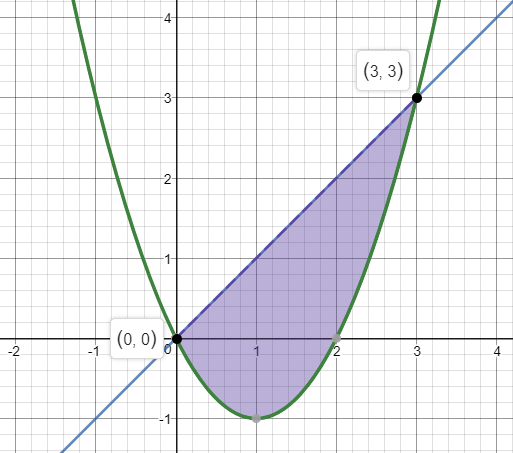
\includegraphics[width=0.6\textwidth]{area5}\end{center}
\solution When inspecting the shaded region, the straight line function, $y=x$ is above the parabola. We could handle this with two separate integrals: find $\int f(x)$ and then subtract $\int g(x)$, or we can simplify and find $\int f(x)-g(x)$:
\begin{tasks}[label-offset=-5em](2)
\task[]\begin{align*}
\text{Area}&=\int_a^b[f(x)-g(x)]dx\\
&=\int_0^3[x-(x^2-2x)]dx\\
&=\int_0^3[-x^2+3x]dx\\
\end{align*}
\task[]\begin{align*}
&=-\frac{x^3}{3}+\frac{3x^2}{2}\Big\vert_0^3\\
&=\left(-9+\frac{27}{2}\right)-0=\frac{9}{2}\text{ units}^2\\
\end{align*}
\end{tasks}
\begin{tcolorbox}
\textbf{Area between functions}\\
Let $f(x)$ be the upper function and $g(x)$ be the lower function, then\\
\[\text{Area }=\int_a^b[f(x)-g(x)]dx\]
\end{tcolorbox}

\clearpage
\example A logo is formed by the shaded area between the cubic function  $ f(x)=4x -x^3$ and a parabola $g(x)=2x-x^2$. The two curves intersects at $x=0$ and $x=2$. Find the shaded area.\\
\begin{multicols}{2}
	\begin{tikzpicture}
	\begin{axis}[
	axis lines=center,
	height=8cm,
	axis on top=true,
	ymax=4,ymin=-4,
	xmax=3,xmin=0,
	xlabel=$x$,
	]
	\addplot [name path =F,<->,domain=-2.3:2.3,thick, samples=200, black] {-x^3+4*x};
	\addplot [name path = G,<->,domain=-2.3:2.3,thick, samples=200, red] {-x^2+2*x};
	\addplot[pattern=north west lines, pattern color=blue!50]fill between[of=F and G, soft clip={domain=0:2}];
	\end{axis}
	\end{tikzpicture}
	\columnbreak
\\	\solution Identify the top curve $f(x)$ and subtract the bottom $g(x)$:
	\begin{align*}
	\mathrm{Shaded \hspace{0.2cm}area}&=\int_{a}^{b}(f(x)-g(x))dx\\
	&=\int_{0}^{2}\left((4x-x^3)-(2x-x^2)\right)dx\\
	&=\int_{0}^{2}\left((2x-x^3+x^2)\right)dx\\
	&=\left[\left(2\frac{x^2}{2}-\frac{x^4}{4}+\frac{x^3}{3} \right)\Big|_{0}^2\right]\\
	&=\left[\left(4-\frac{16}{4}+\frac{8}{3}\right)-(0)\right]\\
	&=\frac{8}{3} \,\, \mathrm{units}^2
	\end{align*}
\end{multicols}

%---------------------------------------------------
% Volume
%---------------------------------------------------
\section{Volume}
If a function is revolved around an axis it creates a volume between the axis and the function. Similar to how if we integrate a function, it results in an area --- if we integrate an \textit{area} it results in a volume.

\begin{multicols}{2}
	\example A connector was obtained by revolving the function $f(x)={0.3x+1}$ around the $x$-axis for $0\leq x \leq 5$. Calculate the volume of the connector.
\begin{center}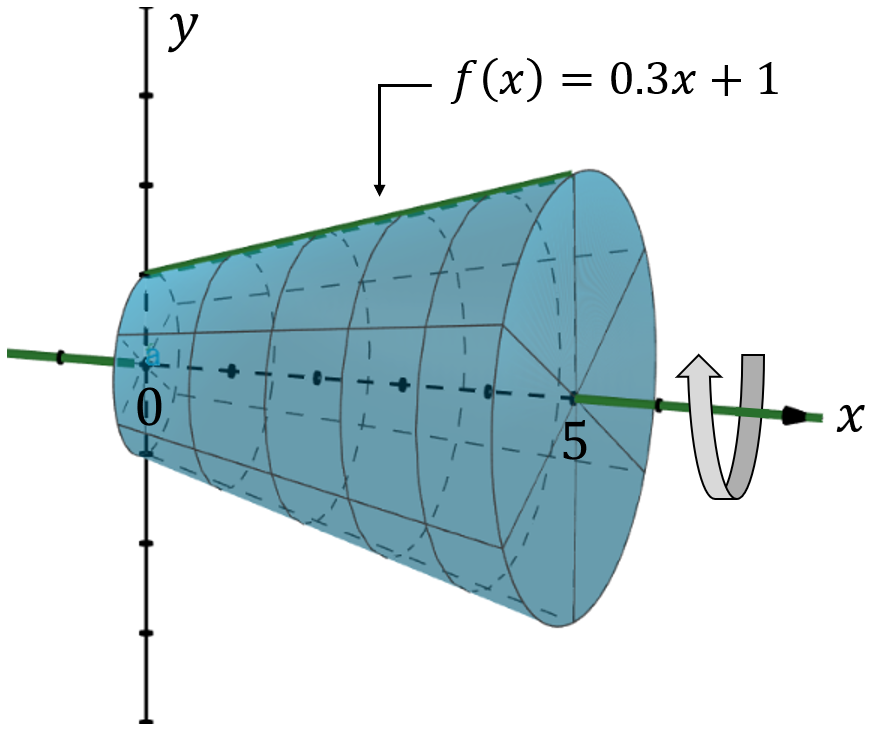
\includegraphics[width=8cm]{solids1}\end{center}
\columnbreak
\solution\\ Given the function of the outer boundary of the shape, we must square the function and integrate this result.\\
\begin{align*}
\mathrm{volume}&=\int_{a}^{b}\pi[f(x)]^2 dx\\
&=\pi\int_0^5\left(0.3x+1\right)^2 dx\end{align*}
Use the power rule and chain rule to integrate:\\
\[=\pi \frac{ (0.3x+1)^3}{0.3(3)} \Big|_0^5\]
Evaluate at the boundary points:\\
\begin{align*}
&=\frac{10\pi}{9}\left[\left(\frac{5}{2}\right)^3-1\right]=\frac{65\pi}{4}\\
&\approx 51.05 \text{ units}^3
\end{align*}
\end{multicols}

\clearpage
The previous example used the disc-method to calculate a volume. Beginning with a rectangular section of width $\Delta x$, and length $f(x)$, just like the Riemann Sum for calculating area on page~\pageref{fig:riemann}. This height becomes a radius when rotated around an axis of revolution, labelled $R$ below. The \textit{volume} of a single disc is $\pi R^2\Delta x$. 
\begin{center}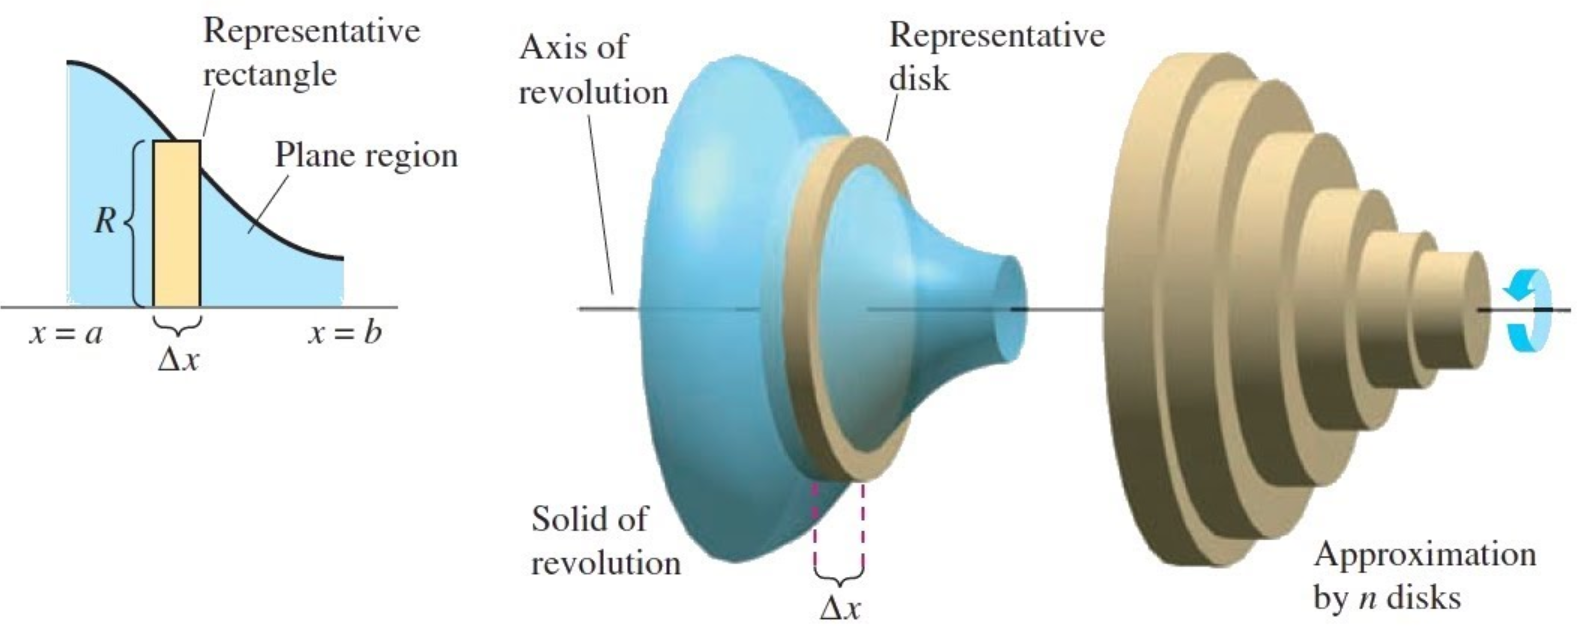
\includegraphics[width=\textwidth]{discMethod}\end{center}
Finding the volume of all the discs involves integrating over the length of the axis from $a$ to $b$.\[\text{Volume}=\int \pi R^2 \Delta x\] The radius is the function evaluation, $f(x)$, and lowercase delta, $\delta$, means infinitesimal thin discs as the number of them goes to infinity, $n\rightarrow\infty$,  we can generalize the formula for volume:
\begin{tcolorbox}
	\textbf{Volume rotated around the $x$-axis}
	\[ \text{Volume} = \int_{a}^{b} \pi y^2 dx = \int_{a}^{b} \pi (f(x))^2 dx\]
	\textbf{Volume rotated around the $y$-axis}
	\[ \text{Volume} = \int_{c}^{d} \pi x^2 dy =\int_{c}^{d} \pi (f(y))^2 dy  \]
\end{tcolorbox}


\example Fluorescent and incandescent light bulbs are often filled with the inert gas krypton. Find the volume of krypton gas required to fill the bulb shown.\vspace{0.4cm}\\ 
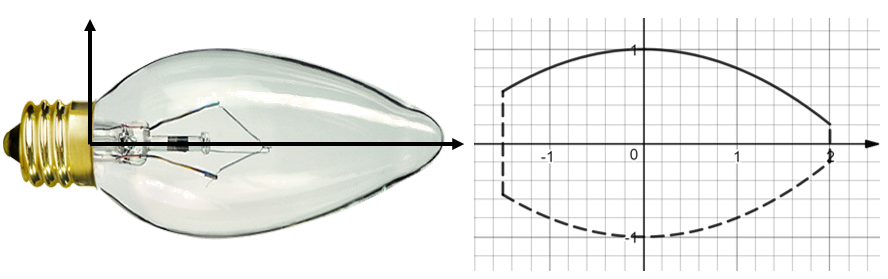
\includegraphics[width=15cm]{bulb}\\
The function has been estimated to be:\\
\[f(x)=1-\frac{x^2}{5}\qquad\text{ for } -1.5\leq x \leq 2\text{ cm}\] 
\solution You will have to calculate $\left(1-\frac{x^2}{5}\right)^2$ before integrating\\
	\begin{align*}
	\text{volume}&=\int_{a}^{b}\pi[f(x)]^2 dx\\
	&=\pi\int_{-1.5}^{2}\left(1-\frac{x^2}{5}\right)^2 dx\\
	&=\pi\int_{-1.5}^{2}\left(\frac{x^4}{25}-\frac{2x^2}{5}+1\right)dx\\
	&=\pi\left(\frac{x^5}{125}-\frac{2x^3}{15}+x\right)  \Bigg|_{-1.5}^2\\
	&=\pi\left[\left(\frac{32}{125}-\frac{16}{15}+2\right)-\left(-0.06075--0.45-1.5\right)\right]=2.3\pi\approx 7.23\, \text{ cm}^3\end{align*}
\\	
\begin{multicols}{2}
\examq Calculate the volume of the container found by rotating the curve $y=\sqrt{x^3}$ around the $y-$axis for $0\leq y \leq 5$.\\

Here the volume is created by rotation about the $y$-axis, and therefore we need to adjust our formula. First we will solve the equation $y=\sqrt{x^3}$ for $x$, and then integrate.
\columnbreak
\begin{center}
		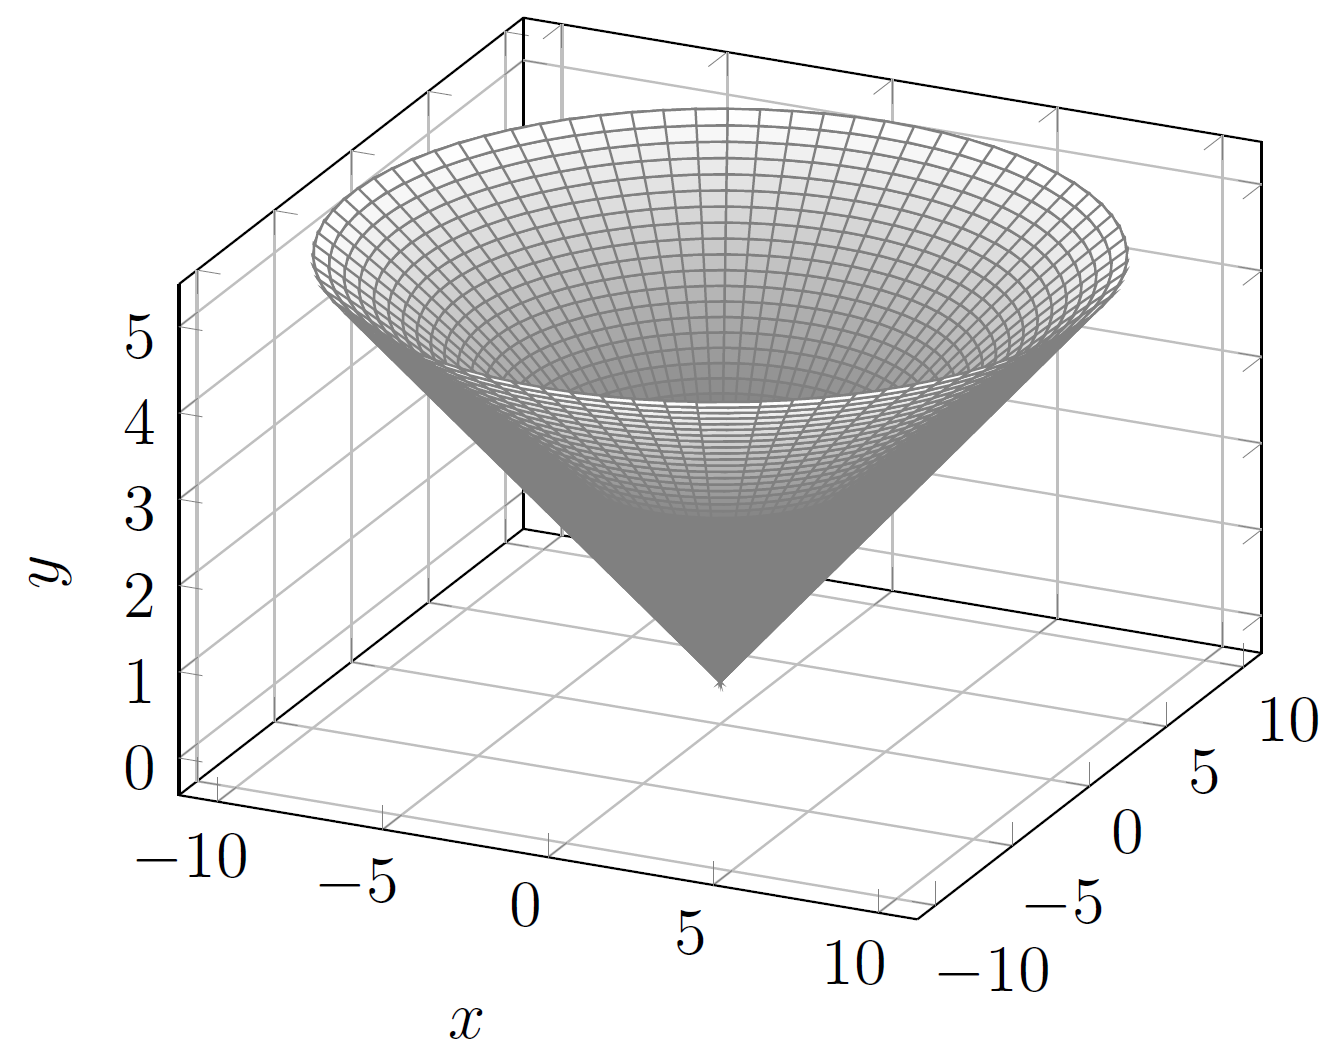
\includegraphics[width=0.5\textwidth]{funnel.png}
\end{center}
\end{multicols}

\solution Volume $=\int_{a}^{b} \pi f(y)^2 dy$\\
\begin{multicols}{2}
Rearrange the function to isolate $x$:
	\begin{align*}
	y&=\sqrt{x^3}\\
	y^2&=x^3\\
	\sqrt[3]{y^2}&=x\end{align*}
Integrate to find volume:\\
	\begin{align*}V&=\pi\int_{0}^{5} (y^{\frac{2}{3}})^2\,dy\\
	&=\pi\int_{0}^{5} y^{\frac{4}{3}}\,dy\\
	&=\pi\frac{y^{\frac{7}{3}}}{\frac{7}{3}}\bigg\vert_{0}^{5}\\
	&=\frac{3\pi}{7}5^{\frac{7}{3}}-0\\
	&\approx 57.6 \,\,\mathrm{units}^3
	\end{align*}
\end{multicols}

%---------------------------------------------------
% Integration by Substitution
%---------------------------------------------------
\section{Integration by Substitution}
Earlier we stated that every differentiation rule leads to an integration rule. The chain rule for differentiation leads to the substitution rule for integration, i.e. the \emph{substitution rule for integration}. 

A series of examples will illustrate how integration by substitution works.

\example Find the integral: $\int 2 x \sqrt{1 +x^{2}}\; d x$.\medskip\\
\solution This cannot be integrated using the techniques discussed so far. This is an example of a function that can be integrated using the substitution rule. They are often recognised by noting the presence of a composite function; the $\sqrt{1 +x^{2}}$ can be seen as $\sqrt{u}$ where the $1+x^2$ under the root is replaced by a new variable.

Let $u=1+x^2$. The integral now becomes $\int 2x\sqrt{u}\; dx$. This is not yet ready because there are two different variables: $u$ \textbf{and} $x$. Lets differentiate the new equation:
\begin{align*}
u&=1+x^2\\
\frac{du}{dx}&=2x
\end{align*}
And we can isolate the $dx$ with the intention of replacing it in the original integral, so $\displaystyle dx=\frac{du}{2x}$.

If we now look back at the original question we are ready to substitute expressions containing $u$ for expressions containing $x$.
\begin{align*}
\int 2 x \sqrt{1 +x^{2}}\; d x &  = \int \sqrt{u} \cdot 2 x\; d x \\
 &  = \int \sqrt{u}\cdot \cancel{2x}\; \frac{du}{\cancel{2x}}\\
 &  = \int u^{\frac{1}{2}}\; d u \\
 &  = \frac{u^{\frac{1}{2} +1}}{\frac{1}{2} +1}= \frac{2}{3}\sqrt[2]{u^3}+C
 \end{align*}
 One last step is to switch back to the original variable $x$. Make the final substitution $u=1+x^2$.
 \[ = \frac{2 \sqrt{\left (1 +x^{2}\right )^{3}}}{3} +C \]
 
The Substitution Rule can be stated formally as follows. If $u =g (x)$ is a differentiable function whose range is an interval $I$ and $f$ is continuous on $I$, then $\int f \left (g \left (x\right )\right ) g^{ \prime } \left (x\right )\; d x =\int f \left (u\right )\; d u$. $d x$ and $d u$ are known as differentials. The Substitution Rule permits us to replace $g^{ \prime } \left (x\right )\; d x$ with $d u$. 

\example Find $\int x \sin  \left (x^{2}\right )\; dx$\medskip\\
\solution Using the procedure from the previous example try $u =x^{2}$. This gives $d u =2 x\; d x\text{.}$
\begin{align*}\int x \sin  \left (x^{2}\right )\; d x &  = \int \sin  \left (x^{2}\right ) \cdot x\; d x \\
 &  = \int \sin(u) \cdot \cancel{x}\cdot\frac{du}{2\cancel{x}} \\
 &  = \frac{1}{2} \int \sin(u)\; d u \\
 &  =  -\frac{1}{2} \cos  u +C \\
 &  =  -\frac{1}{2} \cos  \left (x^{2}\right ) +C\end{align*}

It is clear the challenge of the Substitution Rule is to come up with a suitable substitution. Earlier examples often have fairly obvious substitutions but they can quickly become quite complicated and result in many false starts. \\
\rule{6.8cm}{0.5pt}\\
\example Find $\int \frac{x}{\sqrt{1 -x^{2}}}\; d x$\medskip\\
\solution Let $u =1 -x^{2}$. Then $d u = -2 x\; d x$. So $x\; d x = -\frac{1}{2} d u$. These are now substituted into the original expression
$$\int \frac{x}{\sqrt{1 -x^{2}}}\; d x = -\frac{1}{2} \int \frac{1}{\sqrt{u}}\; d u = -\frac{1}{2} \int u^{ -1/2}\; d u = -\frac{1}{2} \left (2 u^{1/2}\right ) +C = -\sqrt{1 -x^{2}} +C$$

In each of the above 3 examples you could use desmos to compare the original function and the integral to
see if the result is reasonable. For example 3 try graphing the original function $y =\frac{x}{\sqrt{1 -x^{2}}}$ and the integral $y = -\sqrt{1 -x^{2}}$ on the same axes and check the original function represents the slope of the tangent lines to the curve $y = -\sqrt{1 -x^{2}}$. 

\subsection*{Evaluating Definite Integrals by Substitution}
There are two ways to evaluate a definite integral when you have used the Substitution Rule for the integration. 

\textbf{Method 1} Find the indefinite integral then use the Evaluation Theorem. 

\textbf{Method 2} Make the substitution to the integrand and differential (as before) and also use the same substitution to change the limits to those for the new variable (in our questions we usually use $u$). 

\example Evaluate $\int _{0}^{8}\sqrt{x +1}\; d x$. Graphing provides us with the following screen 
\begin{SCfigure}[1][h]
	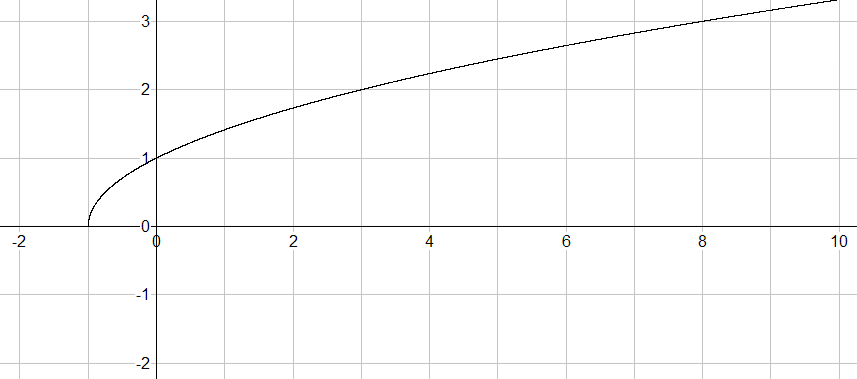
\includegraphics[width=0.7\textwidth]{L4SZ283J}
	\caption*{Figure: The curve is clearly continuous. If we let $u =x +1$ then $u^{ \prime } =1$, this is also continuous.}
\end{SCfigure}

\solution
\textbf{Method 1} 
Substitute $u =x +1$ then $d u =d x$. Substituting these values in the indefinite integral we get
\begin{equation*}\int \sqrt{x +1}\; d x =\int \sqrt{u}\; d u =\frac{2}{3} u^{3/2} +C =\frac{2}{3} \left (x +1\right )^{3/2} +C
\end{equation*}So
\begin{align*}\int _{0}^{8}\sqrt{x +1}\; d x &  = \left .\int \sqrt{x +1}\; d x\right ]_{0}^{8} \\
 &  = \left .\frac{2}{3} \left (x +1\right )^{3/2}\right ]_{0}^{8} \\
 &  = \frac{2}{3} \left (9\right )^{3/2} -\frac{2}{3} \left (1\right )^{3/2} \\
 &  = \frac{2}{3} 27 -\frac{2}{3} 1 \\
 &  = \frac{2}{3} \left (27 -1\right ) =\frac{2}{3} 26 =\frac{52}{3} =17\frac{1}{3}\end{align*}

\textbf{Method 2} 
Again we let $u =x +1$ so $d u =d x$. Also we calculate the new limits for $u$ using $u =x +1$.
\begin{align*}x &  = 0\text{ gives }u =0 +1 =1 \\
x &  = 8\text{ gives }u =8 +1 =9\end{align*}

Now the definite integral is transformed into a definite integral in $u$. 

\begin{align*}\int _{0}^{8}\sqrt{x +1}\; d x &  = \int _{1}^{9}\sqrt{u}\; d u \\
 &  = \left .\frac{2}{3} u^{3/2}\right ]_{1}^{9} \\
 &  = \frac{2}{3} 9^{3/2} -\frac{2}{3} 1^{3/2} \\
 &  = \frac{2}{3} \left (27 -1\right ) =17\frac{1}{3}\end{align*}

A check on the graph will show that an area of $17\frac{1}{3}$ appears to be reasonable. 

Method 2 is usually preferred as the step where the indefinite integral is first calculated has been neatly incorporated into the method. The difficulty with method 2 is that once the values for $u$ have been calculated the integral is completely transformed and we never return to the original question. We answer a different question that, because of the transformation, has the same answer. This concept might cause confusion. However a graph of the situation shows what has happened.   
\begin{center}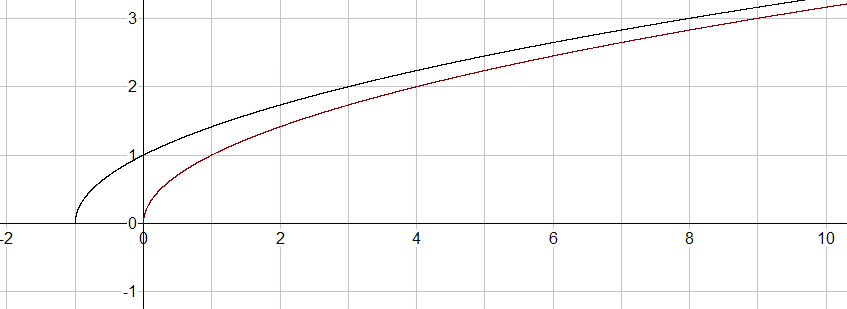
\includegraphics[ width=5.3195in, height=1.9579in]{L4SZ283K}\end{center}
It is clear that the area under the first graph between $0$ and $8$ is the same as the area under the second graph between $1$ and $9$. 

%---------------------------------------------------
% Integration by Parts
%---------------------------------------------------
\section{Integration by Parts}
Recall the rule for the differentiation of a product
\begin{equation*}\frac{d}{d x} \left (f (x) \cdot g (x)\right ) =f (x) \cdot g^{ \prime } (x) +g (x) \cdot f^{ \prime } (x)
\end{equation*}

We can integrate each side and write the process as follows
\begin{align*}f (x) \cdot g (x) &  = \int \left [f (x) \cdot g^{ \prime } (x) +g (x) \cdot f^{ \prime } (x)\right ]\; d x \\
 &  = \int f (x) \cdot g^{ \prime } (x)\; d x +\int g (x) \cdot f^{ \prime } (x)\; d x\end{align*}

This is rewritten in a particular way to become the formula for \emph{integration by parts}.
\begin{align}\int f (x) \cdot g^{ \prime } (x)\; d x &  = f (x) \cdot g (x) -\int g (x) \cdot f^{ \prime } (x)\; d x \tag{1} \\
\text{or}\int f (x) \cdot g^{ \prime } (x)\; d x &  = f (x) \cdot g (x) -\int f^{ \prime } (x) \cdot g (x)\; d x \tag{2}\end{align}

This formula is written in a number of different ways in textbooks. Here
are two ways 

Let $u =f (x)$ and $v =g (x)$ then $d u =f^{ \prime } (x)\; d x$ and $d v =g^{ \prime } (x)\; d x$ so using the substitution rule equation (1) becomes
\begin{equation}\int u\; d v =u v -\int v\; d u\tag{3}
\end{equation}

Let $\int f (x) \cdot g^{ \prime } (x)\; d x$ be regarded as the the integral of the product of two functions then $g =\int g^{ \prime }$. We can write equation (2) as
\begin{tcolorbox}
	\[\int fg'=fg-\int f'g \tag{4}\]
\end{tcolorbox}
Equations (3) and (4) are the common forms that are best to remember.

The success of this method depends on the discovery that a simpler integral results from this process. Sometimes the process results in a worse situation than you started with so should be abandoned. Sometimes you produce a pattern which leads to a solution after 2 or more applications of the integration by parts rule. The patterns that produce solvable problems can be discovered as different questions are tried. 

\example Find $\int x \cos  x\; d x$. This can be seen as the integral of a product. The two functions
are $f (x) =x$ and $g (x) =\cos  x$. So $f^{ \prime } (x) =1$ and $\int g (x) =\sin  x$ are easy to find. Notice though that $f^{ \prime } (x) =1$ gives us a clue that \emph{integration by parts} is going to be a fruitful method. \\
\solution
Using equation (2)
\begin{align*}\int x \cos  x\; d x &  = f (x) \cdot g (x) -\int f^{ \prime } (x) \cdot g (x)\; d x \\
 &  = x \cdot \sin  x -\int 1 \cdot \sin  x\; d x \\
 &  = x \cdot \sin  x -\int \sin  x\; d x \\
 &  = x \cdot \sin  x -\left ( -\cos  x\right ) +C \\
 &  = x\; \sin  x +\cos  x +C\end{align*}
\rule{6.8cm}{0.5pt}\\
\example Use integration by parts to find $\int \ln  x\; d x$. This is a function that has arisen in the course as the integral of $\frac{1}{x}$, however we are now able to use this fact to help with this question. \\
\solution Notice there is only one function here so we have to create two functions by stating $\ln  x =1 \cdot \ln  x$. The two functions are therefore $f (x) =\ln  x$ and $g (x) =1$. Can we find $f^{ \prime }$ and $\int g$? Yes!
\begin{align*}\int \ln  x\; d x &  = \int \ln  x \cdot 1\; d x \\
 &  = \ln  x \cdot x -\int \frac{1}{x} \cdot x\; d x \\
 &  = x\; \ln  x -\int 1\; d x \\
 &  = x\; \ln  x -x +C\end{align*}
\rule{6.8cm}{0.5pt}\\
\example Find $\int e^{x} \cos  x\; d x$ This is an example where a pattern is established and perseverance leads to the solution. \\
\solution Let $f (x) =\cos  x$ and $g (x) =e^{x}$. Can we find $f^{ \prime }$ and $\int g$? Yes!
\begin{align*}\int e^{x} \cos  x\; d x &  = \cos  x \cdot e^{x} -\int  -\sin  x \cdot e^{x}\; d x \\
 &  = e^{x} \cos  x +\int e^{x} \sin  x\; d x\end{align*}

This is an integral that is very similar in appearance to the original question with the $\cos  x$ transformed into $\sin  x$. We continue by repeating the integration by parts process with the new integral
$\int e^{x} \sin  x\; d x$
\begin{align*}\int e^{x} \cos  x\; d x &  = e^{x} \cos  x +\overset{\int e^{x} \sin  x\; d x}{\overbrace{\sin  x \cdot e^{x} -\int \cos  x \cdot e^{x} d x}} \\
 &  = e^{x} \cos  x +e^{x} \sin  x -\int e^{x} \cos  x\; d x\end{align*}

Notice the original integral has now appeared on the right hand side of the equation. We
now simply solve the equation for $\int e^{x} \cos  x\; d x$ and add the constant of integration.
\begin{align*}2 \int e^{x} \cos  x\; d x &  = e^{x} \cos  x +e^{x} \sin  x \\
\int e^{x} \cos  x\; d x &  = \frac{e^{x}}{2} \left (\cos  x +\sin  x\right ) +C\end{align*}

This can easily be verified by differentiating. 

\subsection*{Definite Integrals}
Integration by parts can be combined with the Evaluation Theorem to evaluate definite integrals. If
we assume $f^{ \prime }$ and $g^{ \prime }$ are continuous then we can use the Evaluation Theorem and write equation (1) as follows
\begin{equation}\int _{a}^{b}f (x) \cdot g^{ \prime } (x)\; d x =\left .f (x) \cdot g (x)\right ]_{a}^{b} -\int _{a}^{b}g (x) \cdot f^{ \prime } (x)\; d x\tag{5}
\end{equation}

\example Evaluate $\int _{0}^{1}x e^{x}\; d x$. A graph of $y =x e^{x}$ shows the area required and gives us an idea of the answer to expect. 
\begin{center}
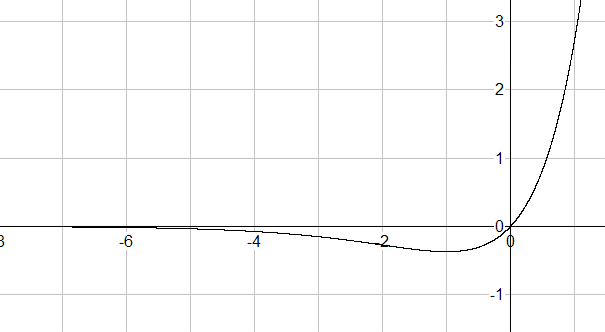
\includegraphics[ width=4.7374in, height=2.6126in,]{L4SZ283M}
\end{center}
\solution Notice $x$ becomes simpler when differentiated and $e^{x}$ is unchanged when it is integrated
\begin{align*}\int _{0}^{1}x e^{x}\; d x &  = \left .x e^{x}\right ]_{0}^{1} -\int _{0}^{1}1 \cdot e^{x}\; d x \\
 &  = \left .x e^{x}\right ]_{0}^{1} -\left .e^{x}\right ]_{0}^{1} \\
 &  = \left (\left (1 e^{1}\right ) -\left (0 e^{0}\right )\right ) -\left (e^{1} -e^{0}\right ) \\
 &  = e^{1} -e^{1} +e^{0} \\
 &  = e^{0} =1\end{align*}


%---------------------------------------------------
% Applications of Integration
%---------------------------------------------------
\section{Applications of Integration}

\subsection*{Rectilinear Motion}
We will use integration to analyse the motion of an object moving in a straight line. Let
the position function for the object be $s =f (t)$ where $t$ is the time. The velocity function is $v (t) =s^{ \prime } (t)$. Therefore the position function is the integral of the velocity function. Also
the acceleration function is $a (t) =v^{ \prime } (t)$ so the velocity function is the integral of the acceleration function. We can obtain
the position function from the acceleration function by integrating twice. This process will generate
two constants of integration so we need two additional pieces of information to find the particular solution. Usually
$s (0)$ and $v (0)$ are given. 

\example A particle moves in a straight line with an acceleration of $a (t) =4 t +2$. If the initial velocity is $ -4 \mbox{cm}$/$\mbox{s}$ and the initial displacement is $5 \mbox{cm}$, find the position function. 

\solution \begin{multicols}{2}
As $v^{ \prime } (t) =a (t) =4 t +2$ we can integrate $a (t)$ to obtain $v (t)$
\begin{align*}v(t)&=\int a(t)dt\\
&=\int (4t+2)dt\\
&=4 \frac{t^{2}}{2} +2 t +C_{1} \\
&=2 t^{2} +2 t +C_{1}
\end{align*}

Substitute $t =0$ since we know the initial velocity $v(0)=-4$:
\begin{align*}v (0) &  = 2 \cdot 0^{2} +2 \cdot 0 +C_{1}\\
C_{1} &  =  -4\text{ and therefore} \\
v (t) &  = 2 t^{2} +2 t -4\end{align*}

Integrate $v (t)$ to obtain $s (t)$:
\begin{align*}s(t)&=\int v(t)dt\\
&=2 \frac{t^{3}}{3} +2 \frac{t^{2}}{2} -4 t +C_{2} \\
 &  = \frac{2}{3} t^{3} +t^{2} -4 t +C_{2}\end{align*}

Substitute $t =0$ because we are given the initial displacement i.e. $s (0) =5$
\begin{align*}s (0) &  = \frac{2}{3} \cdot 0^{3} +0^{2} -4 \cdot 0 +C_{2}\\
C_{2} &  = 5\text{ and therefore} \\
s (t) &  = \frac{2}{3} t^{3} +t^{2} -4 t +5\end{align*}
\end{multicols}

\rule{6.8cm}{0.5pt}\\

The gravitational force near the Earth's surface that produces a downwards acceleration is about $-9.8$ m/s$^2$, represented by the vector quantity, $\vec{g}$.\\
\example A ball is thrown vertically upwards with a speed of $24.5 \mbox{m}$/$\mbox{s}$ from the edge of a cliff that is $147 \mbox{m}$ above the ground. 
\begin{tasks}[column-sep=30pt](2)
\task Find the position function. 
\task Find the time when the ball reaches its maximum height. 
\task Find the maximum height above the ground. 
\task When does the ball hit the ground? \end{tasks}

\clearpage\solution
\begin{multicols}{2} \textbf{(a)} It is usual to choose the positive direction
to be upwards this means that $\vec{g}=-9.8$ m/s$^2$. Integrating the acceleration function yields the velocity function.
\begin{align*}v(t)&=\int a(t)dt\\
&  =\int -9.8dt\\
&=-9.8t +C_{1}\end{align*}
Substituting $v (0) =24.5$ we get that $C_{1} =24.5$
\begin{equation*}v (t) = -9.8 t +24.5
\end{equation*}
Because $s^{ \prime } (t) =v (t)$ we integrate $v (t)$
\begin{equation*}\int v(t)=s(t)=-9.8 \frac{t^{2}}{2} +24.5 t +C_{2}
\end{equation*}
Substitute $s (0) =147$. We get $C_{2} =147$.
\begin{equation*}\therefore s(t) = -4.9 t^{2} +24.5 t +147
\end{equation*}
This expression will hold true until the ball is acted on by an external force (hits the ground).

\textbf{(b)} The maximum height is reached when\\ $v (t) =0$; for a moment the vertical velocity will be zero before it begins to fall.
\begin{align*} -9.8 t +24.5 &  = 0 \\
24.5 &  = 9.8 t \\
t &  = \frac{24.5}{9.8}=2.5\text{ s}\end{align*}

\textbf{(c)} The maximum height is found by substituting $t =2.5$ into $s(t)$
\begin{align*}s (2.5) &  =  -4.9 \cdot 2.5^{2} +24.5 \cdot 2.5 +147 \\
 &=177.6 \text{ m}\end{align*}

\textbf{(d)} The ball hits the ground when the displacement, $s(t) =0$.
\begin{align*}-4.9 t^{2} +24.5 t +147 &  = 0 \\
t^{2} -5 t -30 &  = 0\end{align*}
Solve for $t$ using the quadratic formula: 
\begin{align*}t &  = \frac{5 \pm \sqrt{25 -4 \times 1 \times  -30}}{2} \\
 &  = \frac{5 \pm \sqrt{145}}{2} \\
 &  =8.5\text{ s, or }-3.5\text{s}\end{align*}
The negative result will be discarded, however, represents a solution to the parabola in an algebraic sense. We did not test whether the value of $t$ when $v (t) =0$ gives a maximum or minimum. A maximum can be assumed knowing that $-9.8$ m/s$^2$ has a negative coefficient. 
\end{multicols}

\subsection*{Work}
The strategy we use to allow us to apply calculus to a problem in engineering is the same as we used to evaluate areas. The
physical quantity is divided up into a large number of small parts, each one approximately equal to the theoretical quantity it represents. These
are then summed and a limit taken as the number of small parts, $n \rightarrow \infty $. This process allows us to evaluate the resulting integral. 

You
will recall that from Newton's Second Law of Motion
\begin{equation}F =m a =m \frac{d^{2} s}{d t^{2}}\tag{1}
\end{equation}

Where $s (t)$ is the position function, $m$ is the mass of an object and $F$ is the force required to produce an acceleration of $a$. (Where $a =\frac{d^{2} s}{d t^{2}}$). 

We usually measure mass in kilograms ($\mbox{kg}$), distance in metres ($\mbox{m}$) and force in newtons ($\mbox{N}$) \linebreak\relax ($N =k g \cdot m/s^{2}$). If the acceleration is constant then the force to produce that acceleration will also
be constant. 

Work = force $ \times $ distance or
\begin{equation}W =F d\tag{2}
\end{equation}If $F$ is in newtons and $d$ is in metres then $W$ is in newton-metres. One newton-metre is called a\linebreak\relax joule ($\mbox{J}$).

\example A mass of 3.5 kg lifted 0.5 m requires a force of $\displaystyle F =m a =3.5 \times 9.8 =34.3 \mbox{N}$. This is the force required to counter the force exerted by gravity. Calculate the work done.\\
\solution The work done is calculated using equation 2
\begin{equation*}W =F d =34.3 \times 0.5 =17.15 \text{ J}
\end{equation*}

If the force is variable this formula can no longer be applied. Let the force acting on an object as it moves along the $x$-axis in a positive direction from $a$ to $b$ be $f (x)$, where $f$ is a continuous function of $x$. Divide the interval from $a$ to $b$ into $n$ subintervals of width $ \Delta x$ where $ \Delta x =\frac{b -a}{n}$. For simplicity we let the end points of these subintervals be $x_{0}$, $x_{1}$, $x_{2}$, ..., $x_{n}$ We select the $i^{t h}$ subinterval and select a representative $x$-value in this interval $x_{i}^{ \ast }$. The work done when we move the object from $x_{i -1}$ to $x_{i}$ is
\begin{equation*}W_{i} \approx f (x_{i}^{ \ast })  \Delta x
\end{equation*}

The total work done is
\begin{equation}W =\sum _{i =1}^{n}f (x_{i}^{ \ast })  \Delta x\tag{3}
\end{equation}

As we did with area we find the limit as $n \rightarrow \infty $ of this sum. As this is a Riemann sum the limit is a definite integral
\begin{equation}W =\sum _{i =1}^{n}f (x_{i}^{ \ast })  \Delta x =\int _{a}^{b}f (x)\; d x\tag{4}
\end{equation}
\rule{6.8cm}{0.5pt}\\
\example If the force on a particle is given by the equation $f (x) =3 x^{2} -2 x \text{ N}$, how much work is done moving the particle from $x =2$ to $x =3$?

\solution The graph of $f (x) =3 x^{2} -2 x$ shows that for the interval $\left [2 ,3\right ]$ the area is above the $x$-axis.
\begin{align*}W &  = \int _{a}^{b}f (x)\; d x \\
 &  = \int _{2}^{3}\left (3 x^{2} -2 x\right )\; d x \\
 &  = \left .3 \frac{x^{3}}{3} -2 \frac{x^{2}}{2}\right ]_{2}^{3} \\
 &  = \left .x^{3} -x^{2}\right ]_{2}^{3} \\
 &  = \left (3^{3} -3^{2}\right ) -\left (2^{3} -2^{2}\right ) \\
 &  = 18 -4 =14\text{ J}\end{align*}
\clearpage
%\rule{6.8cm}{0.5pt}\\
\examq Hooke's Law states that the force required to maintain a spring stretched $x$ units beyond its natural length is proportional to $x$, the spring displacement in meters, such that $f (x) =k x$ where $k$ is the spring constant and $f$ the force. This law holds provided $x$ does not get too large. \medskip\\
The work required to stretch the spring can be calculated by integrating the force function:
\[W=\int_{a}^{b}f(x) \, dx\,. \]
Find the work done in stretching a spring from 12 cm to 17 cm given that it takes 4 newtons of force to stretch the spring from 10 cm to 12 cm. \\
\solution\medskip\\
First you will need to find the spring constant $k$:
\begin{align*}f(x)&=kx\\
4\,\text{N}&=k(0.12-0.10)\\
k&=\frac{4}{0.02}=200\,\,\frac{\text{newtons}}{\text{meter}}
\end{align*}
Integrate the force function for find the work done in stretching the spring:
\begin{align*}
W&=\int_{0.12}^{0.17}200x\,dx\\
&=100x^2\Big\vert_{0.12}^{0.17}\\
&=100(0.17^2-0.12^2)\\
&=1.45 \text{ J}
\end{align*}
\clearpage
%---------------------------------------------------
% Chapter Exercises in a separate file
%---------------------------------------------------
\section{Chapter Exercises}
\subimport{}{5IntegrationExercises}


 



